\begin{problem}{경주}
	{standard input}{standard output}
	{3 seconds}{128 megabytes}{}
	
	지구이웨에서 매년 개최되는 자전거 경주가 올해에도 어김없이 개최된다. 지구이웨의 사이클리스트(자전거 타는 사람)들은 긴 거리를 다닌다. 모터사이클리스트(오토바이 타는 사람)들은 사이클리스트와 계속 마찰을 빚어왔고, 이 경주를 사보타주하기로 결심한다.
	
	지구이웨는 $n$개의 교차로가 있고, 단방향 도로로 연결되어있다. 신기하게도, 이 도로망에는 사이클이 없다. -- 만약 교차로 $u$에서 교차로 $v$로 갈 수 있다면, 교차로 $v$에서 교차로 $u$로는 가지 못한다.	

	경주는 지구이웨에 도로를 따라 열릴것이다. 모터사이클리스트들은 그들의 불타오르는 바이크를 타고 대회가 열리는 교차로 중 하나에 가서 그 교차로를 막을 것이다. 전국 사이클리스트 협회는 당연히 다른 경로로 대회를 열 것이고, 이 경로가 매우 짧아서 사이클리스트들이 자신의 놀라운 지구력을 뽐낼 수 없을 수도 있다. 이는 모터사이클리스트들의 계획이다. 그들은 한 교차로를 막아서 최장거리를 제일 짧게 만들고 싶다.
	
	\InputFile
	입력의 첫째 줄에는 지구이웨의 교차로의 수와 도로의 수를 의미하는 $n$, $m$이 공백 하나로 구분되어 주어진다.($2 \le n \le 500,000$, $1 \le m \le 1,000,000$) 교차로는 1번부터 $n$번까지 번호가 붙어 있다. 다음 $m$개의 줄의 $i$번째 줄에는 두 정수 $a_i$, $b_i$가 공백 하나로 구분되어 주어진다. ($1 \le a_i, b_i \le n$, $a_i \neq b_i$) 이것은 교차로 $a_i$부터 $b_i$까지가 단방향 도로로 연결 되어 있다는 것을 의미한다.
	
	
	
	\OutputFile
	
	프로그램은 첫째 줄에 두 개의 공백 하나로 구분된 정수를 출력하여야 한다. 첫번째 수는 모터사이클리스트들이 막아야 하는 교차로의 번호를 출력하고, 두번째 수는 사이클리스트들이 경주를 할 수 있는 가장 긴 경로의 도로의 수를 출력한다. 답이 여러개인 경우, 아무 답이나 출력해도 좋다.
	
	
	\SubtaskWithCost{1}{33}
	\begin{itemize}
		\item 모든 도로 $i$에 대해, $a_i < b_i$.
	\end{itemize}
	
	\SubtaskWithCost{2}{67}
	추가 제한 조건이 없다.
	
	
	
	\Examples
	
	\begin{example}
		\exmp{
			6 5
			1 3
			1 4
			3 6
			3 4
			4 5
			
		}{%
		1 2
		
	}%
\end{example}

\Note

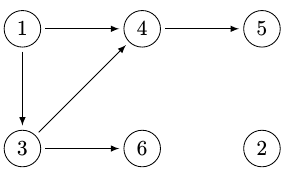
\includegraphics[width=0.3\linewidth]{raj.png}

\end{problem}

